\documentclass[svgnames]{article}
\usepackage[utf8]{inputenc}
\usepackage{amsmath}
\usepackage{amssymb}
\usepackage{mathrsfs}
\usepackage{mathtools}
\newtheorem{mydef}{Given}
\newtheorem{mytheorem}{Theorem}
\usepackage{enumitem}
\usepackage{venndiagram}
\usepackage{smartdiagram}
\usepackage{caption}
\usepackage{subcaption}
%\usepackage[framed,numbered,autolinebreaks,useliterate]{mcode}
\usepackage{pgfplots}
%\usepackage{tkiz}



\usepackage{listings}
\usepackage{color}

\definecolor{dkgreen}{rgb}{0,0.6,0}
\definecolor{gray}{rgb}{0.5,0.5,0.5}
\definecolor{mauve}{rgb}{0.58,0,0.82}

\lstset{frame=tb,
  language=Java,
  aboveskip=3mm,
  belowskip=3mm,
  showstringspaces=false,
  columns=flexible,
  basicstyle={\small\ttfamily},
  numbers=none,
  numberstyle=\tiny\color{gray},
  keywordstyle=\color{blue},
  commentstyle=\color{dkgreen},
  stringstyle=\color{mauve},
  breaklines=true,
  breakatwhitespace=true,
  tabsize=3
}
\usepackage{graphicx}
\graphicspath{ {./images/} }
%\renewcommand{\theenumi}{\Alph{enumi}}
\newenvironment{amatrix}[1]{%
  \left(\begin{array}{@{}*{#1}{c}|c@{}}
}{%
  \end{array}\right)
}

\newenvironment{tolerant}[1]{%
  \par\tolerance=#1\relax
}{%
  \par
}


\title{Statistical Methods: Mid Term}
\author{Cameron McIntyre}
\date{October 2018}

\begin{document}

\maketitle

\section{Question 1}
 A researcher finds that, of 982 men who died in 2002, 221 died from some heart disease.
Also, of the 982 men, 334 had at least one parent who had some heart disease. Of the latter
334 men, 111 died from some heart disease. A man is selected from the group of 982. Given
that neither of his parents had some heart disease, find the conditional probability that this
man died of some heart disease.

\textbf{Answer:}
\newline
Define Events
\newline
H - Died of Heart Disease.
\newline
P - Parents Have Heart Disease 
 $$ P(H|\bar{P})=\frac{P(H\cap\bar{P})}{P(\bar{P})} = \frac{\frac{221-111}{982}}{\frac{982-334}{982}}=.1697$$


\section{Question 2}
 At the beginning of a certain study of a group of persons, 15\% were classified as heavy
smokers, 30\% as light smokers, and 55\% as nonsmokers. In the five-year study, it was
determined that the death rates of the heavy and light smokers were five and three times that
of the nonsmokers, respectively. A randomly selected participant died over the five-year
period; calculate the probability that the participant was a nonsmoker.

\textbf{Answer:}
\newline
Events:
\newline
H - Heave smoker. $P(H) = .15$
\newline
L - Light Smokers. $P(L) = .30$
\newline
N - Non Smoker $P(N) = .55$
\newline
We also know
\newline
$P(D|N)=X$
\newline
$P(D|L)=3X$
\newline
$P(D|H)=5X$
\newline
We need to find $P(N|D)$.

$$P(N|D)=\frac{P(D|N)\cdot P(N)}{P(D)}=\frac{X \cdot .55}{\sum_{i \in (N, L, H)} P(D|i)P(i)}=\frac{X \cdot .55}{X\cdot .55 + 3X\cdot .3 + 5X\cdot .15}$$

$$P(N|D) = \frac{X \cdot .55}{X(.55 + 3\cdot .3 + 5\cdot .15)}= \frac{.55}{2.2}=.25$$


\section{Question 3}
 An insurance company sells an automobile policy with a deductible of one unit. Let X be the
amount of the loss for a policy, with X having a probability density function

$$P_{X}(x) = .9,\ if\ x = 0$$
$$P_{X}(x) = \frac{c}{x},\ if\ x = 1,2,3,4,5,6$$

\begin{enumerate}[label = (\alph*)]
\item
Determine c to make the probability density valid:

$$1 = .9 + \sum_{1}^{6}\frac{c}{x} = .9 + c(\frac{1}{1}+\frac{1}{2}+\frac{1}{3}+\frac{1}{4}+\frac{1}{5}+\frac{1}{6})\leftrightarrow .1 =  c \cdot 2.45  $$
 $$  c = \frac{.1}{2.45}$$
 \newline
 \newline
Therefore our distribution becomes:
$$P_{X}(x) = .9,\ if\ x = 0$$
$$P_{X}(x) = \frac{1}{2.45}\cdot \frac{1}{x},\ if\ x = 1,2,3,4,5,6$$

 
\item 
Expected value of the amount of insurance a company must pay:
\newline
\newline
 The payout function is $0 , X\in(0,1)$ and $X-1, X \in (2,3,4,5,6)$.
 \newline
 \newline
 $$E[Payout] = 0*.9 + 0*\frac{1}{2.45}\cdot \frac{1}{1}+1*\frac{1}{2.45}\cdot \frac{1}{2}+2*\frac{1}{2.45}\cdot \frac{1}{3}+3*\frac{1}{2.45}\cdot \frac{1}{4}+4*\frac{1}{2.45}\cdot \frac{1}{5}+5*\frac{1}{2.45}\cdot \frac{1}{6}$$
 $$E[Payout]  = 1.44898 $$

\end{enumerate}


\section{Question 4}
 Suppose that 2000 points are selected independently and at random from the unit square
$\{0\leq x \leq1,0\leq y\leq1\}$. Let W equal the number of points that fall into $A = X^2 +Y^2 <1$

\begin{enumerate}[label = (\alph*)]
\item
How must W be distributed?
\newline
\newline
The points are distributed uniformly over the unit square. The area that we care about is in the unit circle between $0 \leq \theta \leq \frac{\pi}{2}, 0 \leq r \leq 1$. The probability of a single dot being within that area is going to be the ratio of the areas because the dots are uniformly distributed. 

$$Area\ of\ Unit\ Square =1 * 1 = 1$$
$$Area\ of\ Circle \ in\ unit\ square =\int_{0}^{\frac{\pi}{2}}\int_{0}^{1}r drd\theta =\int_{0}^{\frac{\pi}{2}}\frac{1}{2}d\theta= \frac{\pi}{4} $$
Therefore the probabiltiy of being within the area A is $\frac{\pi}{4}$
\newline
\newline
The probability of a single dot being in the intersection of the unit circle and the unit square is a bernoulli trial with probability $p = \frac{\pi}{4}$. The number of dots within that area can be thought of as a binomial distribution with a successful probability $p = \frac{\pi}{4}$. Because there are 2000 bernoulli trials, each of which are independent and identically distributed. We can use the central Limit Theorem, because the margin of error in convergence is very small for such a large value of N. Also large factorials can become computationally inefficient. 
\newline
\newline
We have estimates for $\mu$ and $\sigma$.
\newline
$\mu=NP=2000*\frac{\pi}{4}=1570.797$
\newline
$\sigma = \sqrt{np(1-p)} = \sqrt{2000\cdot \frac{\pi}{4} \cdot (1-\frac{\pi}{4})}=18.36$
\newline
There for $W\sim N(1570.797, 18.36)$

\item 
What is the mean and standard deviation for W?
\newline
\newline
As we calculated for the distribution above.
\newline
$$ \mu = n*p = 2000 * \frac{\pi}{4}=1570.797$$
\newline
$$ \sigma = \sqrt{n*p(1-p)} = \sqrt{2000 * p * (1-p)}=18.36$$

\end{enumerate}

\section{Question 5}
Let the random variable X be equal to the number of days that it takes a high-risk driver to
have an accident. Assume that X has an exponential distribution. If $P(X<50) = 0.25$, compute
$P(X>100|X>50)$.
\newline
\newline
\textbf{Answer:}

We rely on the Markovian Property (memoryless-ness) of the exponential distribution. In essence for an exponential random variable $P(s+t < X | t < X ) =P(s < X )$.
\newline
So,
$$P(100< X | 50 < X ) = P(50+50 < X | 50 < X ) =P(50 < X ) = 1 - P( X < 50)=1-.25=.75 $$
\newline
\newline
\newline
\textbf{Alternative Solution:}
\newline
We solve for $\lambda$.

$$.25 = 1- e^{-\lambda 50} \leftrightarrow \lambda = -1* \frac{ln(.75)}{50} \leftrightarrow \lambda =  0.005753641$$

$$ P(X>100|X>50)= \frac{P(X>100)\cap P(X>50)}{P(X>50)} = \frac{e^{-\lambda* 100}}{e^{-\lambda* 50}}=e^{-\lambda* 50} = .75$$

\section{Question 6}
A painting contractor was contracted to paint 25 housing units. However, to cut corners the
contractor watered down the paint and failed to give a second coat in 10 of the units. A housing
unit inspector sampled 5 units at random and would be able to tell if the painting job was not
according to specifications. Assume the business model is to approve the work if there is no
more than 20\% found on inspection to be subpar. What is the probability that the contractor?s
work is approved?
\newline
\newline
\textbf{Answer:}
This Inspectors selection of a sub par house is distributed hyper-geometrically. If we define the random variable H to be the number of houses selected that fail the inspection, we are interested in $P(H\leq1)$.
\newline
\newline
We are interested in this quantity because 20\% of the five houses selected is 1. Therefore at maximum he can select 1 faulty house out of the maximum of 5 houses he selects.

$$P(H \leq 1)= P(H=0) + P(H=1) = \frac{\binom{5}{0}\binom{20}{5}}{\binom{25}{5} }+\frac{\binom{5}{1}\binom{20}{4}}{ \binom{25}{5}}=.313439$$ 

\section{Question 7}
Two admirers of a new worker in the office will ask the new worker out according to a pdf of $\frac{4}{x^5}$, $1<x<\infty$ where X is measured in weeks. If the admirers act independently,
determine 
\begin{enumerate}[label = (\alph*)]
\item
The pdf for the maximum wait to be asked out by both and 
\item 
The expected time to be asked out by both.
\end{enumerate}
\textbf{Answer:}
\newline
\newline
\begin{enumerate}[label = (\alph*)]
\item
We know from the text $f_{ymax}(y)=n(F(y))^{n-1}f_Y{y}$.
\newline
So,
$$F_{X}(x)=\int_{1}^{x}\frac{4}{x^5}dx=-\frac{1}{x^4}\Big|^{x}_{1}=1-\frac{1}{x^4}$$
Therefore,
$$f_{Xmax}(x)=2(1-\frac{1}{x^4})^{1}\frac{4}{x^5}=\frac{8}{x^5} - \frac{8}{x^9}=8(\frac{1}{x^5}-\frac{1}{x^9})$$

\item
The expected value is calculated below:
$$E[X]=\int^{\infty}_{1}xf_{Xmax}(x)=8\int^{\infty}_{1}\frac{1}{x^4}-\frac{1}{x^8}=-8\frac{7x^4-3}{21x^7}\Big|_{1}^{\infty}=-8(0 - \frac{4}{21})=\frac{32}{21}$$
\end{enumerate}

\section{Question 8}
Consider a fair four-sided die numbered $1 - 4$ and a fair six-sided die numbered $1 - 6$, where X is
the number appearing on the four-sided die and Y is the number appearing on the six-sided die.
Define $W=X+Y$ when they are rolled together. Assuming $X$ and $Y$ are independent,
Use the moment generating function technique to find the expectation and variance.
\begin{enumerate}[label = (\alph*)]
\item
Find the moment generating function for W.
First we find 
$$M_{X}(t)=\sum^{4}_{i=1}\frac{e^{ti}}{4}=\frac{1}{4}(e^{1t}+e^{2t}+e^{3t}+e^{4t})$$
Similarly,
$$M_{Y}(t)=\sum^{6}_{i=1}\frac{e^{ti}}{6}=\frac{1}{6}(e^{1t}+e^{2t}+e^{3t}+e^{4t}+e^{5t}+e^{6t})$$
We use a result shown in the textbook that when X and Y are independent and $W =X+Y$ then, $M_{W}(t)= M_{X}(t) \cdot M_{Y}(t)$.
\newline
So,
$$M_{W}(t)=\frac{1}{4}(e^{1t}+e^{2t}+e^{3t}+e^{4t})\cdot \frac{1}{6}(e^{1t}+e^{2t}+e^{3t}+e^{4t}+e^{5t}+e^{6t})$$
$$M_{W}(t)=\frac{1}{24}(e^{1t}+e^{2t}+e^{3t}+e^{4t})\cdot (e^{1t}+e^{2t}+e^{3t}+e^{4t}+e^{5t}+e^{6t})$$
\item 
Find the expectation E(W).
$$E(W)=M_{w}'(t)\Big|_{t=0}$$
$$E(W)=\frac{1}{24}(1e^{1t}+2e^{2t}+3e^{3t}+4e^{4t})\cdot (e^{1t}+e^{2t}+e^{3t}+e^{4t}+e^{5t}+e^{6t})$$
$$+ \frac{1}{24}(e^{1t}+e^{2t}+e^{3t}+e^{4t})\cdot (1e^{1t}+2e^{2t}+3e^{3t}+4e^{4t}+5e^{5t}+6e^{6t})\Big|_{t=0}$$
$$E(W) =\frac{1}{24}(1+2+3+4)\cdot (6) + \frac{1}{24}(4\cdot (1+2+3+4+5+6)$$
$$E(W)=\frac{10}{4}\frac{6}{6}+\frac{21}{6}\frac{4}{4}=\frac{72}{12}=6$$
\item 
Find the variance Var(W). 
\newline
\newline
Firstly, we find the second derivative of the moment generating function.
$$\frac{d}{dt}M_{w}'(t)=\frac{1}{24}\Big[\frac{d}{dt}(1e^{1t}+2e^{2t}+3e^{3t}+4e^{4t})\cdot (e^{1t}+e^{2t}+e^{3t}+e^{4t}+e^{5t}+e^{6t})$$
$$+ (e^{1t}+e^{2t}+e^{3t}+e^{4t})\cdot (1e^{1t}+2e^{2t}+3e^{3t}+4e^{4t}+5e^{5t}+6e^{6t}) \Big]$$
$$=\frac{1}{24}\Big[(1e^{1t}+4e^{2t}+9e^{3t}+16e^{4t})\cdot (e^{1t}+e^{2t}+e^{3t}+e^{4t}+e^{5t}+e^{6t}) $$
$$+(1e^{1t}+2e^{2t}+3e^{3t}+4e^{4t})\cdot  (1e^{1t}+2e^{2t}+3e^{3t}+4e^{4t}+5e^{5t}+6e^{6t}) $$
$$+ (1e^{1t}+2e^{2t}+3e^{3t}+4e^{4t})\cdot (1e^{1t}+2e^{2t}+3e^{3t}+4e^{4t}+5e^{5t}+6e^{6t}) $$
$$+(e^{1t}+e^{2t}+e^{3t}+e^{4t})\cdot (1e^{1t}+4e^{2t}+9e^{3t}+16e^{4t}+25e^{5t}+36e^{6t})\Big] $$
$$E[W^2]=M_{w}''(t)\Big|_{t=0}=\frac{1}{24}\Big[30*6 +10*21 + 10*21 + 4 * 91\Big]=\frac{964}{24}$$
\newline
\newline
To find the variance, we use the variance formula $E[X^2]-E[X]^2 = Var[X]$

$$Var[W]=E[W^2] - (E[W])^2 = \frac{964}{245} - \frac{864}{24}= \frac{100}{24}=4.16$$

\end{enumerate}

\section{Question 9}
Let $f_{X,Y}(x,y)=\frac{4}{3},\ 0 < x <1, x^3 < y <1$.
\begin{enumerate}[label = (\alph*)]
\item
Determine the marginal density $f_X(x).$
\item 
Determine the marginal density $f_Y(y).$
\item
Determine the conditional density density $f_{X|Y}(x|y).$

\end{enumerate}
\textbf{Answer:}

\begin{enumerate}[label = (\alph*)]
\item
$$f_X(x)=\int^{1}_{x^3}\frac{4}{3}dy=\frac{4}{3}y\Big|^{1}_{x^3}=\frac{4}{3}(1-x^3), 0<x<1$$
\item
$$f_Y(y)=\int^{y^{\frac{1}{3}}}_{0}\frac{4}{3}dx=\frac{4}{3}x\Big|^{y^{\frac{1}{3}}}_{0}=\frac{4}{3}y^{\frac{1}{3}},0<y<1$$
\item
Note, by definition:
$$f_{X|Y}(x|y)=\frac{f_{X,Y}(x,y)}{f_Y(y).} = \frac{\frac{4}{3}}{\frac{4}{3}y^{\frac{1}{3}}}=\frac{1}{y^{\frac{1}{3}}} \ We \ need \ to \ add \ boundary \ conditions$$
So since $x > 0$, $$x^3<y<1 \leftrightarrow x < y^{\frac{1}{3}} < 1$$
\[f_{X|Y}(x|y)= \begin{cases} 
      \frac{\frac{4}{3}}{\frac{4}{3}y^{\frac{1}{3}}}=\frac{1}{y^{\frac{1}{3}}} & x < y^{\frac{1}{3}} \\
      0 &  x \geq y^{\frac{1}{3}} \\
   \end{cases}
\]
\end{enumerate}

\section{Question 10}
An urn contains b black balls and r red balls. One of the balls is drawn at random, but when
it is put back in the urn c additional balls of the same color are put in with it. Now suppose that
we draw another ball. Show that the probability that the first ball drawn was black given the
second ball drawn was red is $\frac{b}{b+r+c}$.

\textbf{Answer:}
\newline
\newline
Define $X_1$ to be the first ball drawn.
Define $X_2$ to be the second ball drawn.
$$P(X_1=b|X_2=r)=\frac{P(X_1=b \cap X_2=r)}{X_2=r}$$
$$=\frac{P(X_1=b)*P(X_2=r|X_1=b)}{P(X_2=r|x1=b)P(X_1=b)+P(X_2=r|x1=r)P(X_1=r)}$$

$$=\frac{\frac{b}{b+r}\cdot\frac{r}{b+r+c}}{\frac{r}{b+r+c}\cdot\frac{b}{b+r}+\frac{r+c}{b+r+c}\cdot\frac{r}{b+r}}$$
$$=\frac{\frac{b}{b+r}\cdot\frac{r}{b+r+c}}{\frac{r\cdot(b+r+c)}{(b+r+c)\cdot(b+r)}}$$
$$=\frac{b}{b+r}\cdot\frac{r}{b+r+c}\cdot \frac{(b+r+c)(b+r)}{r(b+r+c)}$$
$$=\frac{r}{b+r+c}$$ 

The result is as desired.

\section{Question 11}
During a visit to a primary care physician's office, the probability of having neither lab work
nor referral to a specialist is 0.21. Of those coming to that office, the probability of having lab
work is 0.41 and the probability of having a referral is 0.53. What is the probability of having
both lab work and a referral?
\textbf{Answer:}
\newline
\newline
Define:
\newline
L is the event of having Lab work ordered.
\newline
R is the event of having a referral to a specialist.
\newline
Find $P(L\cap R)$

$$P(L\cup R)^c = .21 \leftrightarrow  P(L\cup R) = .79$$
$$P(L\cup R) = P(L) + P(R) - P(L\cap R) $$
$$P(L\cap R) = P(A) + P(R) - P(L\cup R)$$
$$P(L\cap R) = .41 + .53 - .79$$
$$P(L\cap R) = .15$$


\section{Question 12}

An elliptical jungle clearing has been identified as a military target for a bombing run. Let the equation for the ellipse (in meters) be $\frac{X^2}{400^2} +\frac{Y^2}{200^2} = 1$. Assume the approach of the bomber will be along the major axis, and the target would be the point $(0, 0)$. Assume also that variation of the drop in the X and Y directions are independent, with $X \sim N(0, 175^2)$ and $Y \sim N(50, 150^2)$, with the bias in Y due to unexpected cross breezes. Any strike within the ellipse is considered a hit. Simulate the probability of hit by using 1000 simulations for the X and Y positions of the bomb impact and determining whether that point is inside the ellipse. 
\newline
\newline
\textbf{Note}: You will likely want to express the equation in terms of X and Y to compare an observed X to the boundary for X and the observed Y to the boundary for Y. I recommend that you first screen the observed X and Y to see if they individually have the proper domain for the ellipse: then see if the point is inside. Turn in your code. Run your simulation of 1000, ten times, and list in increasing order your sample proportions to the hundredths place.
\newline
\newline
\newline
\pagebreak
\textbf{Answer:}-Starts on next page.
\begin{table}[]
\begin{tabular}{llllll}
Trial Number&Accuracy&Hits&Misses &Total&\\
TRIAL 9&0.703&703&297&1000&\\
TRIAL 2&0.704&704&296&1000&\\
TRIAL 7&0.71&710&290&1000&\\
TRIAL 3&0.714&714&286&1000&\\
TRIAL 10&0.718&718&282&1000&\\
TRIAL 1&0.722&722&278&1000&\\
TRIAL 5&0.726&726&274&1000&\\
TRIAL 8&0.728&728&272&1000&\\
TRIAL 4&0.735&735&265&1000&\\
TRIAL 6&0.745&745&255&1000&\\
\end{tabular}
\end{table}
\newline
\textbf{Visualizations Below Code Sample}
\newline
\newline
\newline
\textbf{R SCRIPT:}
\begin{lstlisting}
inside_target <- function(x,y) {
  if (x^2/400^2 + y^2/200^2<= 1){
    return(TRUE)
  }
  else{
    return(FALSE)
  }
}
draw_target <- function(x, s) {
  if ( s == -1){
    return( -200*(1-x^2/(400^2))^(1/2) )
  }
  else{
    return(200*(1-x^2/(400^2))^(1/2))
  }
}

trial_results = c()

for (j in (1:10)) {
  x_coords=rnorm(1000, 0, 175)
  y_coords=rnorm(1000, 50, 150)
  
  hits_x = c()
  hits_y = c()
  misses_x = c()
  misses_y = c()
  
  for (i in (1:1000)){
    if (inside_target(x_coords[i],y_coords[i])){
      hits_x = c(hits_x, x_coords[i])
      hits_y = c(hits_y, y_coords[i])
    }
    else{
      misses_x = c(misses_x, x_coords[i])
      misses_y = c(misses_y, y_coords[i])
    }
  }
  trial_results = c(trial_results,length(hits_x)/1000.000)
  plot(hits_x, hits_y , type = 'p', from=-400,to = 400, add = TRUE, col = 'green',xlim=c(-600,600), ylim=c(-400,400), xlab="Primary Axis ~ N(0, 175^2)",ylab="Secondary Axis ~ N(50, 150^2)",main = paste("Trial", toString(j)[1]))
  points(misses_x, misses_y , type = 'p', from=-400,to = 400, add = TRUE, col = 'red',xlim=c(-600,600), ylim=c(-600,600))
  curve(draw_target(x,-1),from=-400,to = 400, add = TRUE, xlim=c(-600,600), ylim=c(-400,400), xlab="Primary Axis ~ N(0, 175^2)",ylab="Secondary Axis ~ N(50, 150^2)")
  curve(draw_target(x,1),from=-400,to = 400, add = TRUE, xlim=c(-600,600), ylim=c(-400,400), xlab="Primary Axis ~ N(0, 175^2)",ylab="Secondary Axis ~ N(50, 150^2)")
  
}
\end{lstlisting}
\textbf{TRIAL 1}
\newline
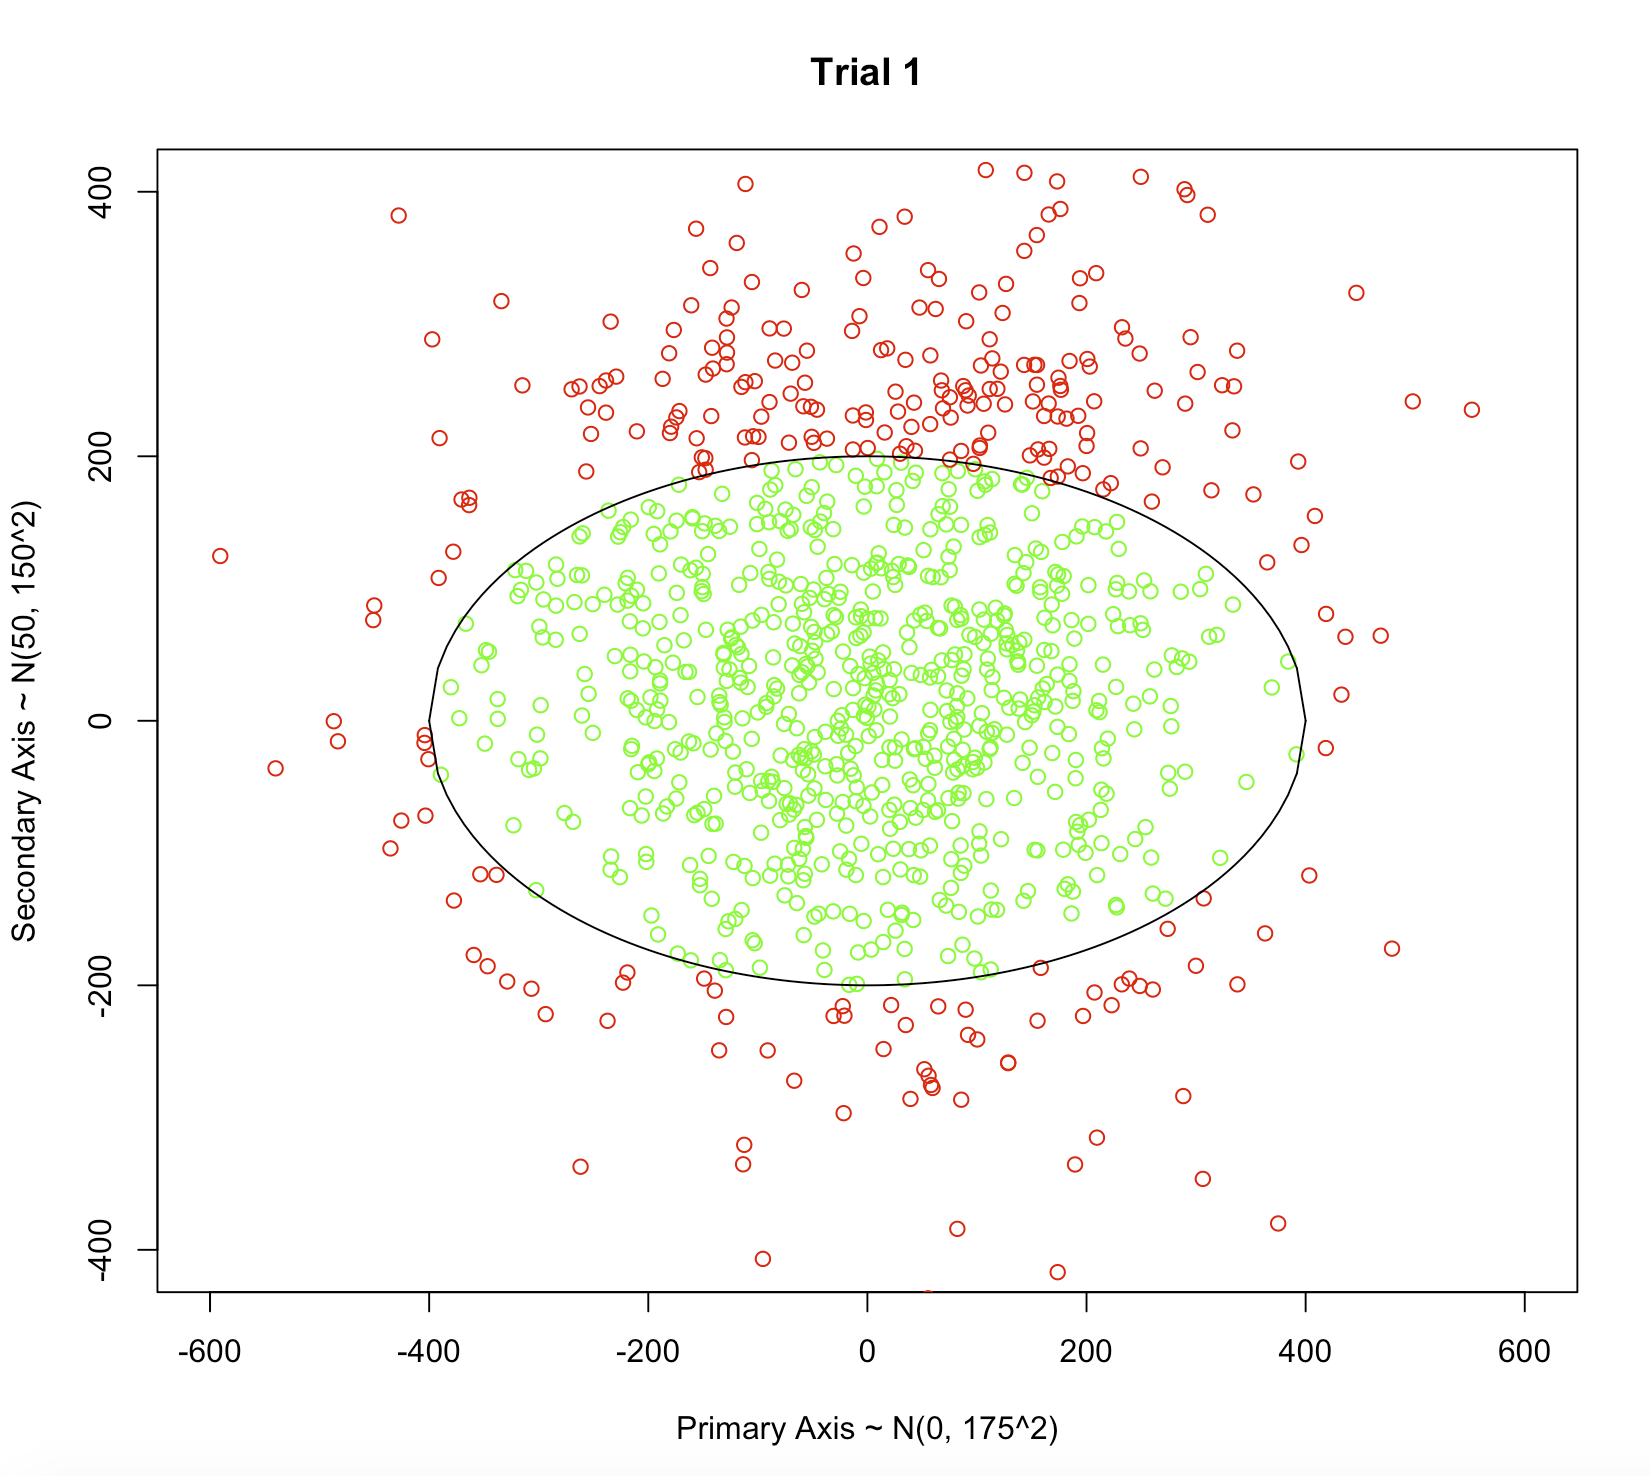
\includegraphics[scale=.30]{trial1}

\textbf{TRIAL 2}
\newline
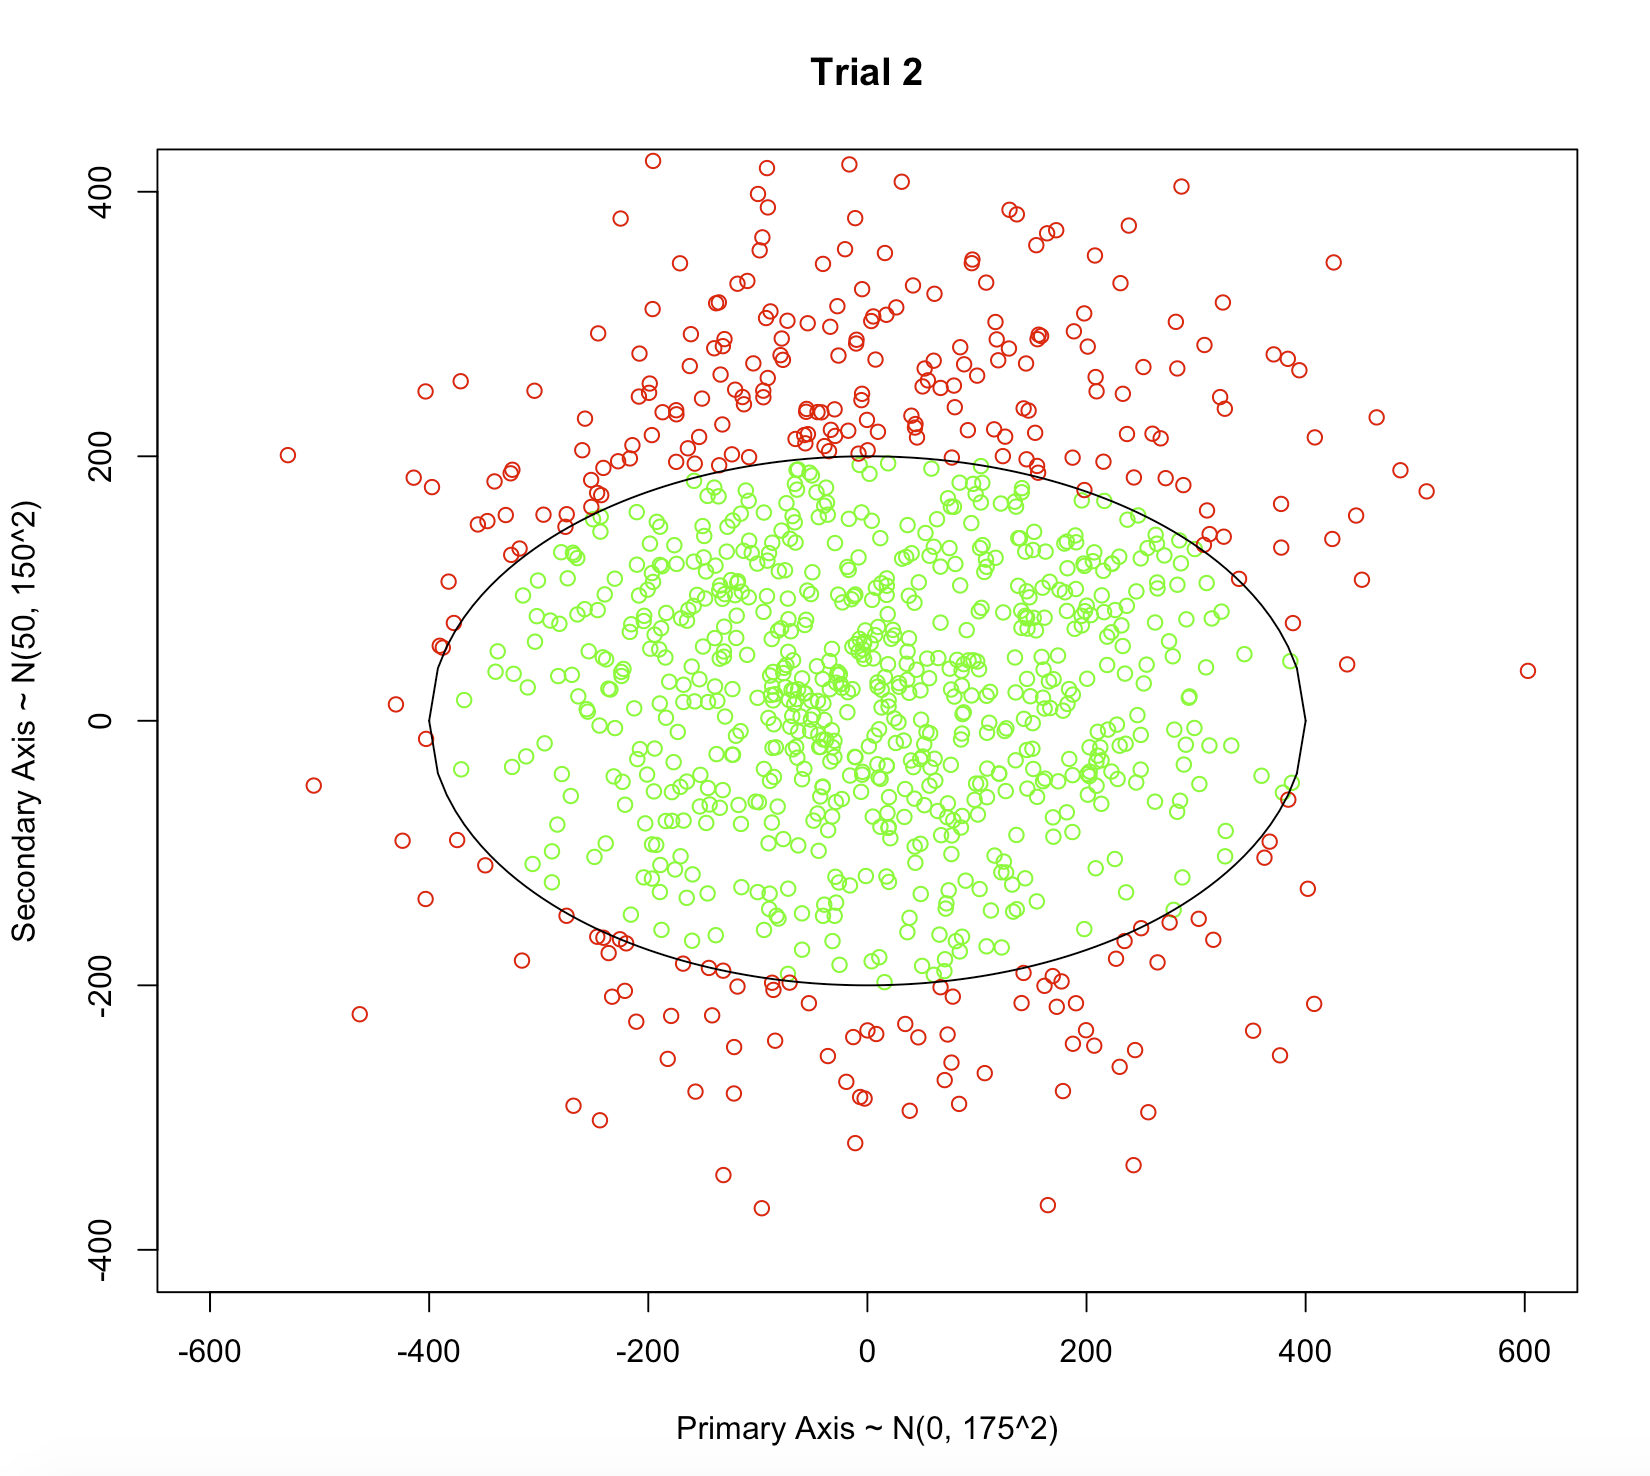
\includegraphics[scale=.30]{trial2}

\textbf{TRIAL 3}
\newline
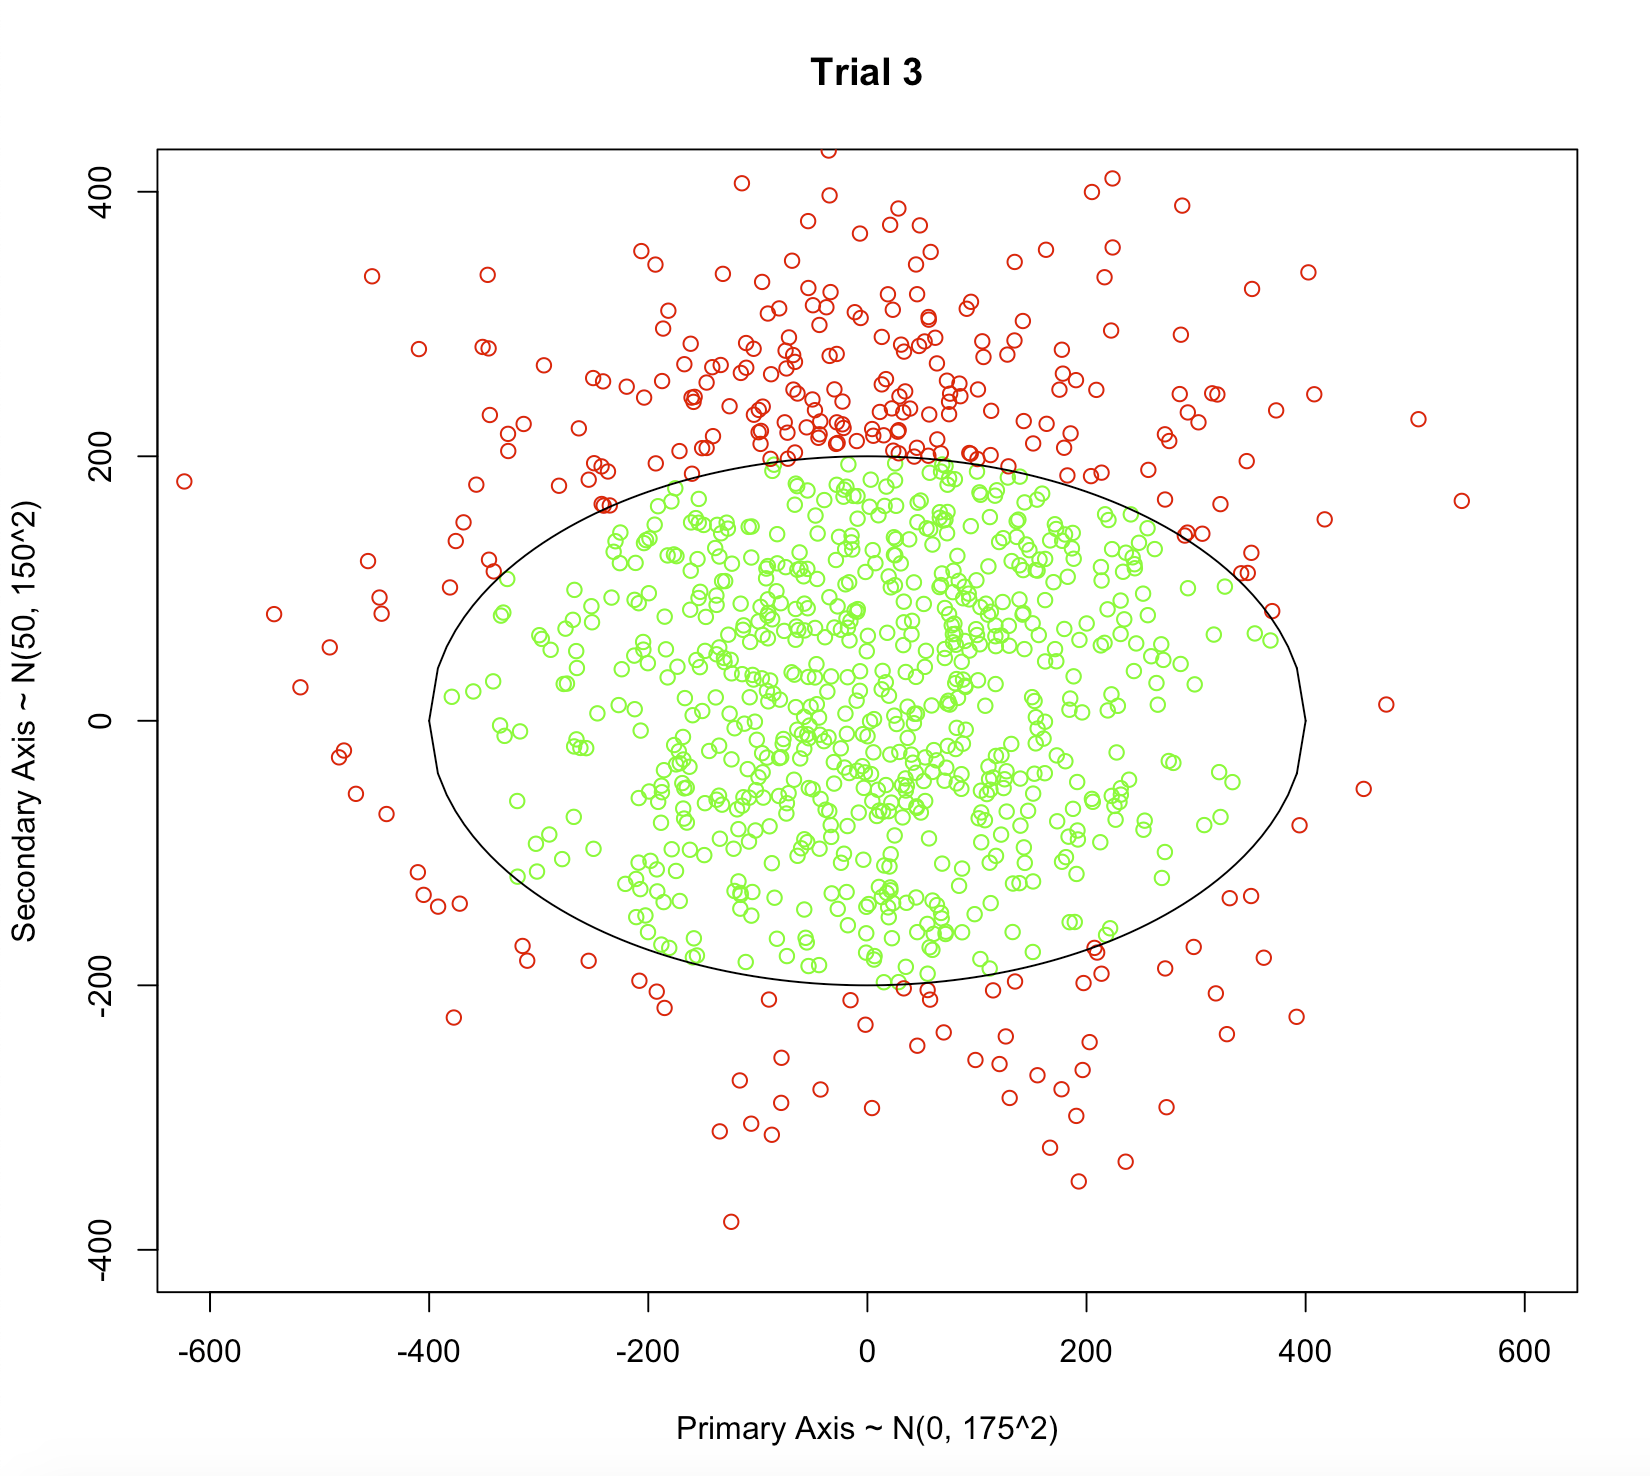
\includegraphics[scale=.35]{trial3}

\textbf{TRIAL 4}
\newline
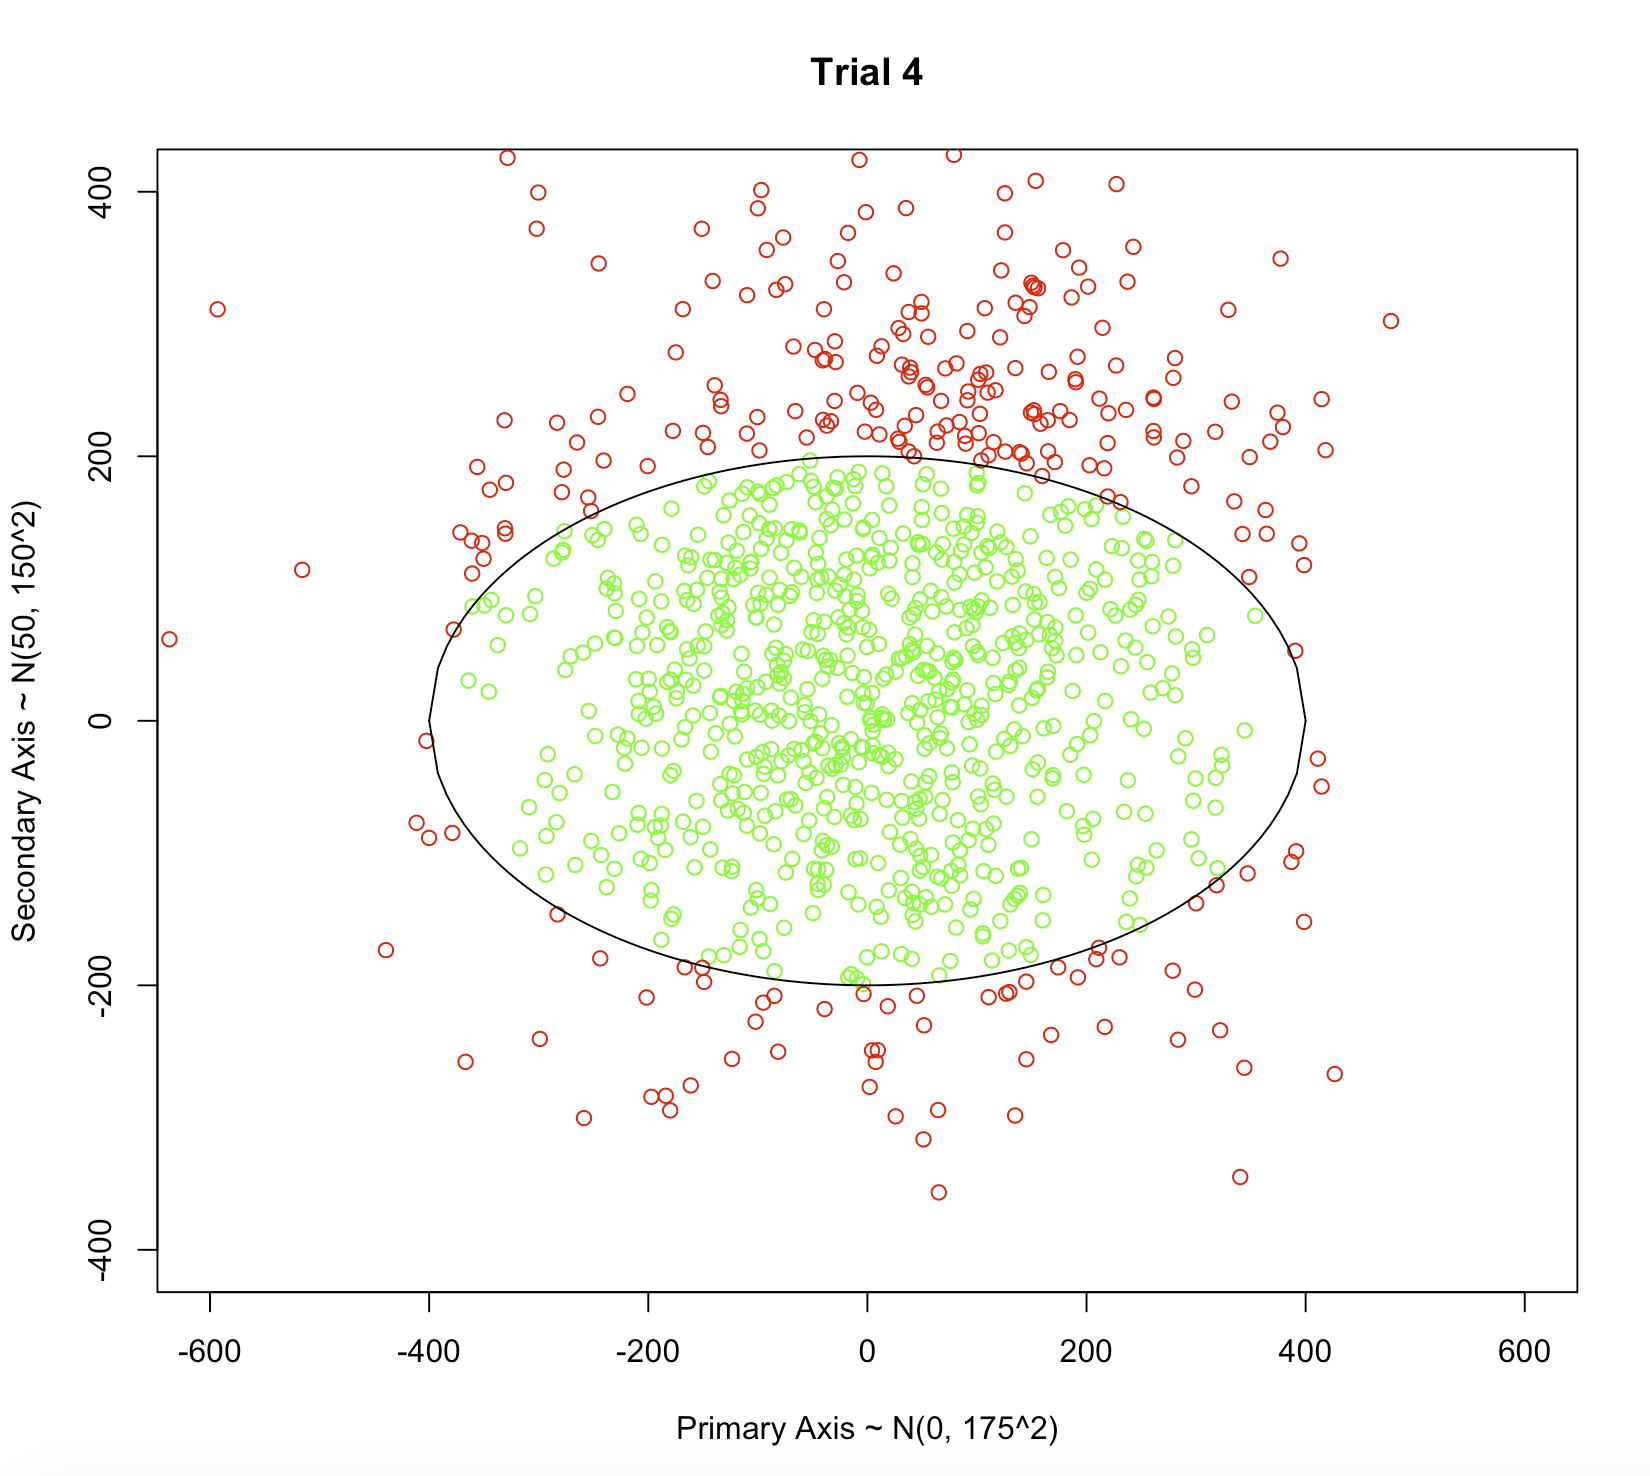
\includegraphics[scale=.35]{trial4}

\textbf{TRIAL 5}
\newline
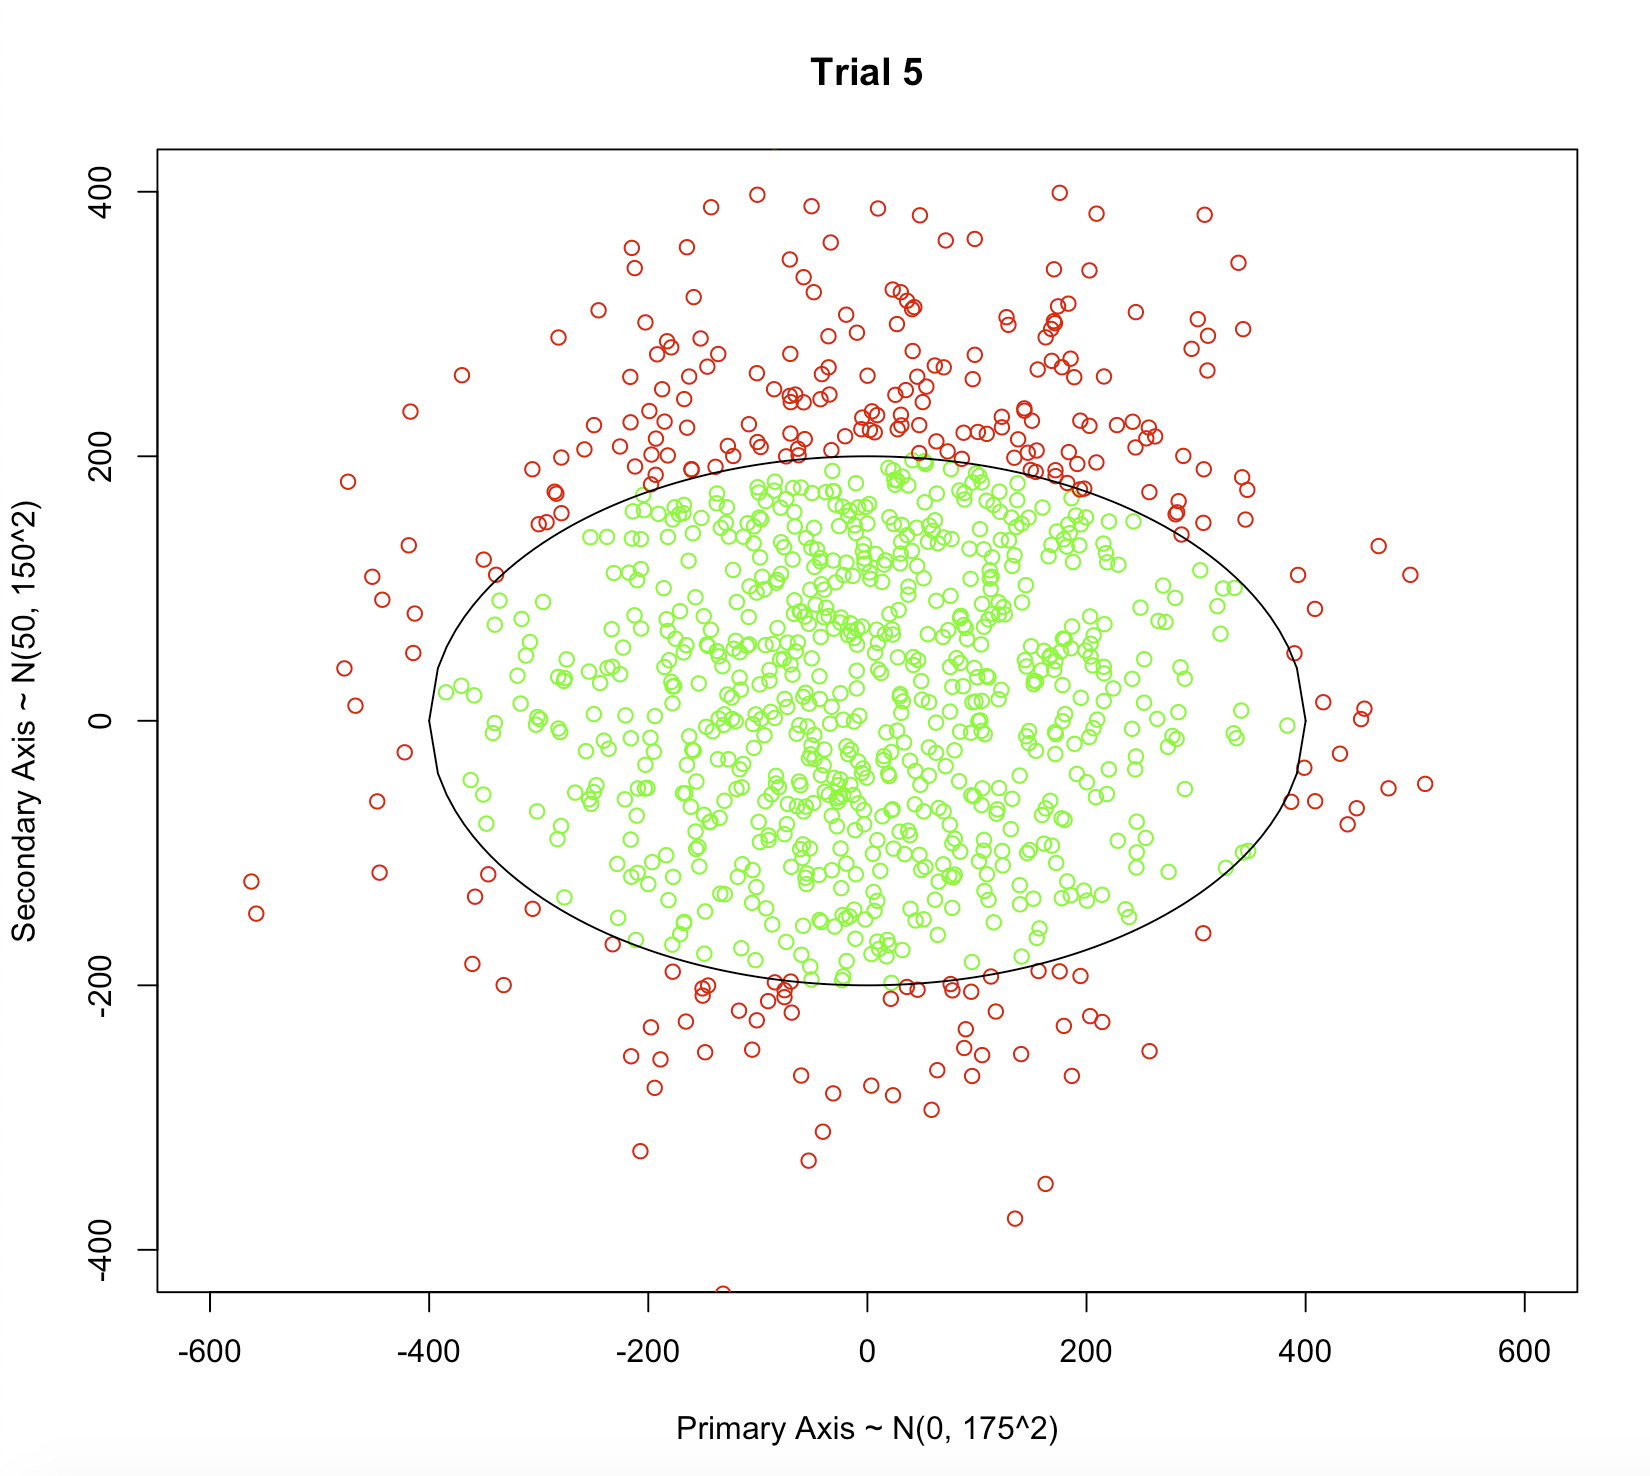
\includegraphics[scale=.35]{trial5}

\textbf{TRIAL 6}
\newline
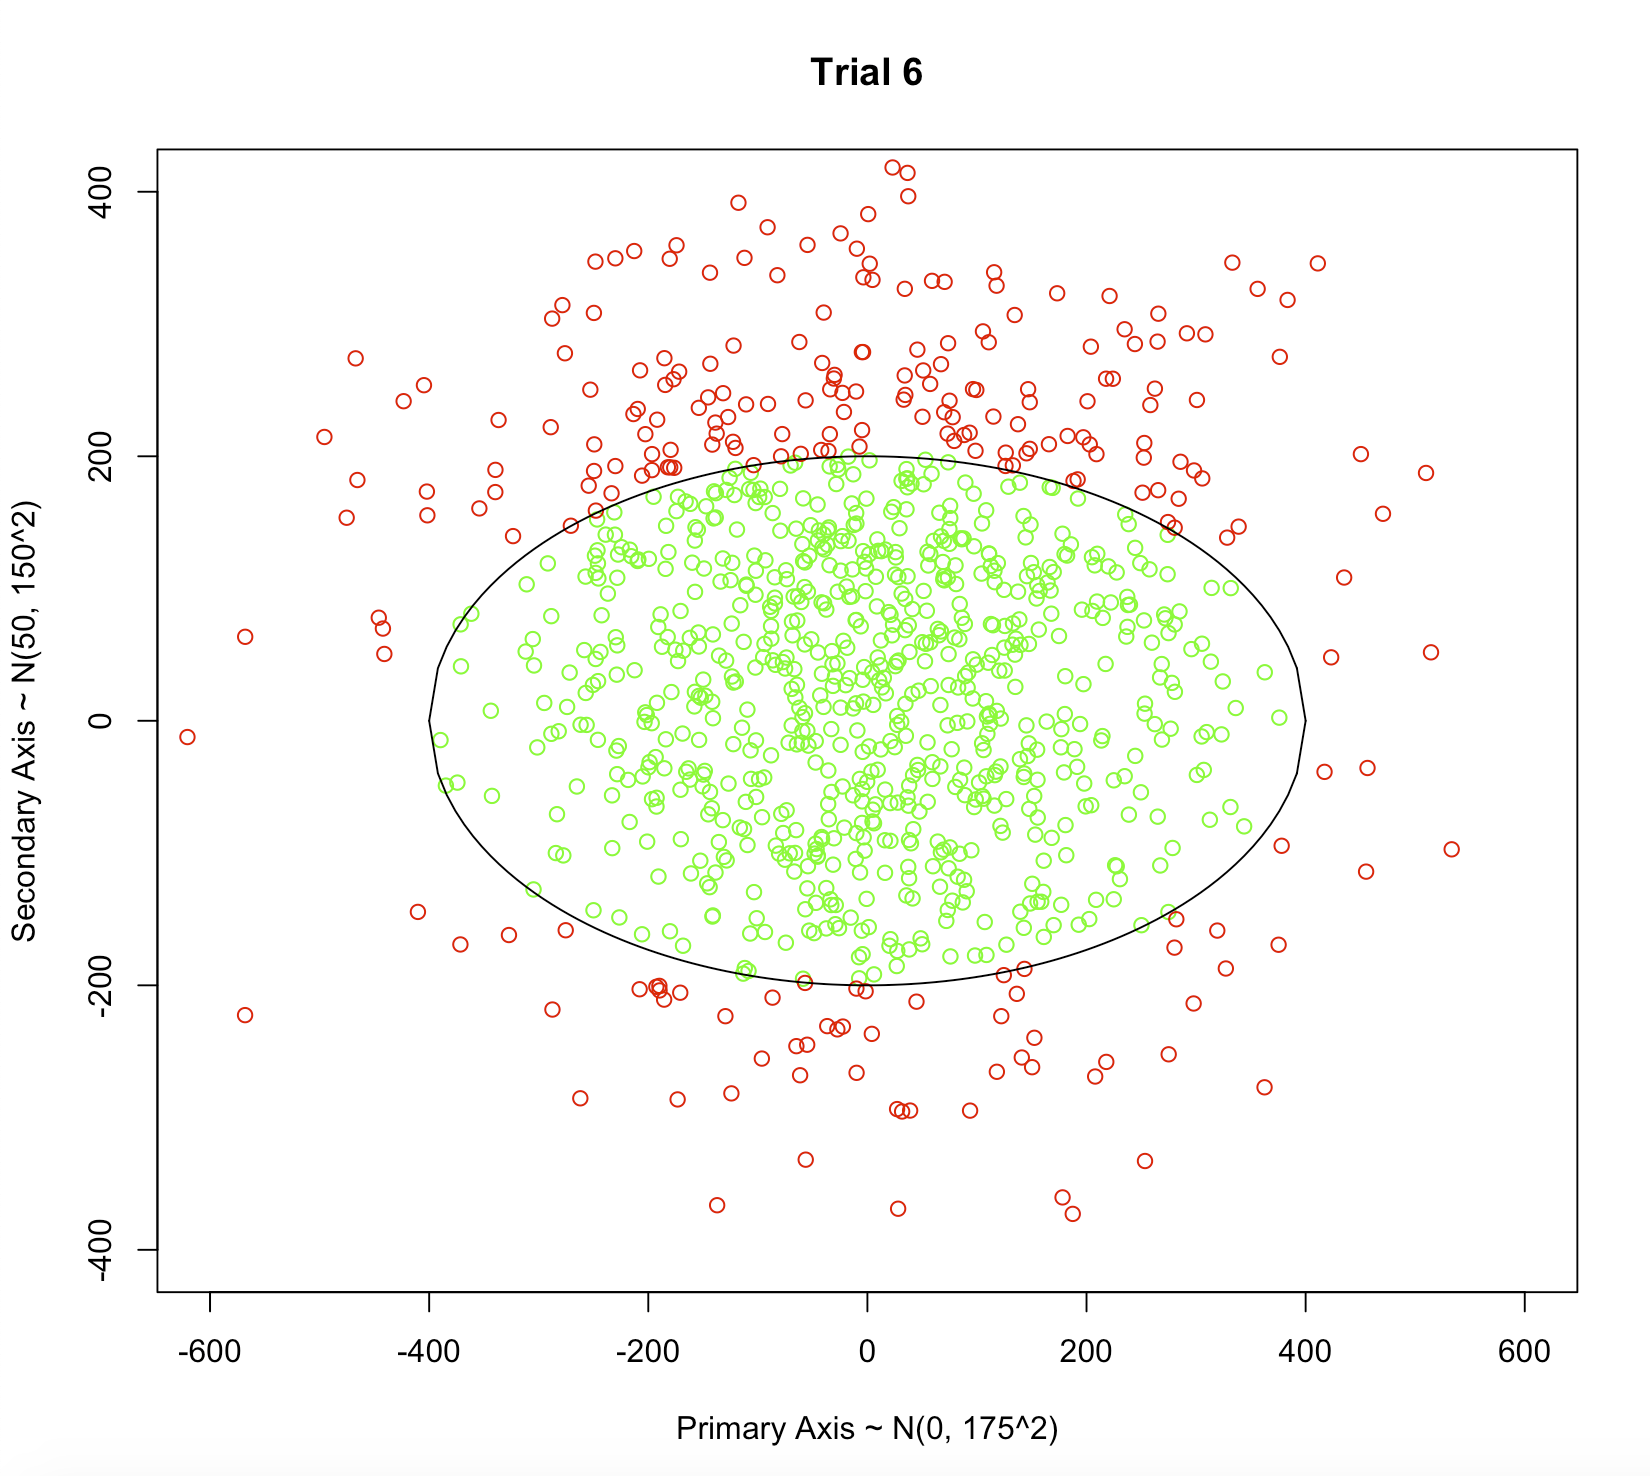
\includegraphics[scale=.35]{trial6}

\textbf{TRIAL 7}
\newline
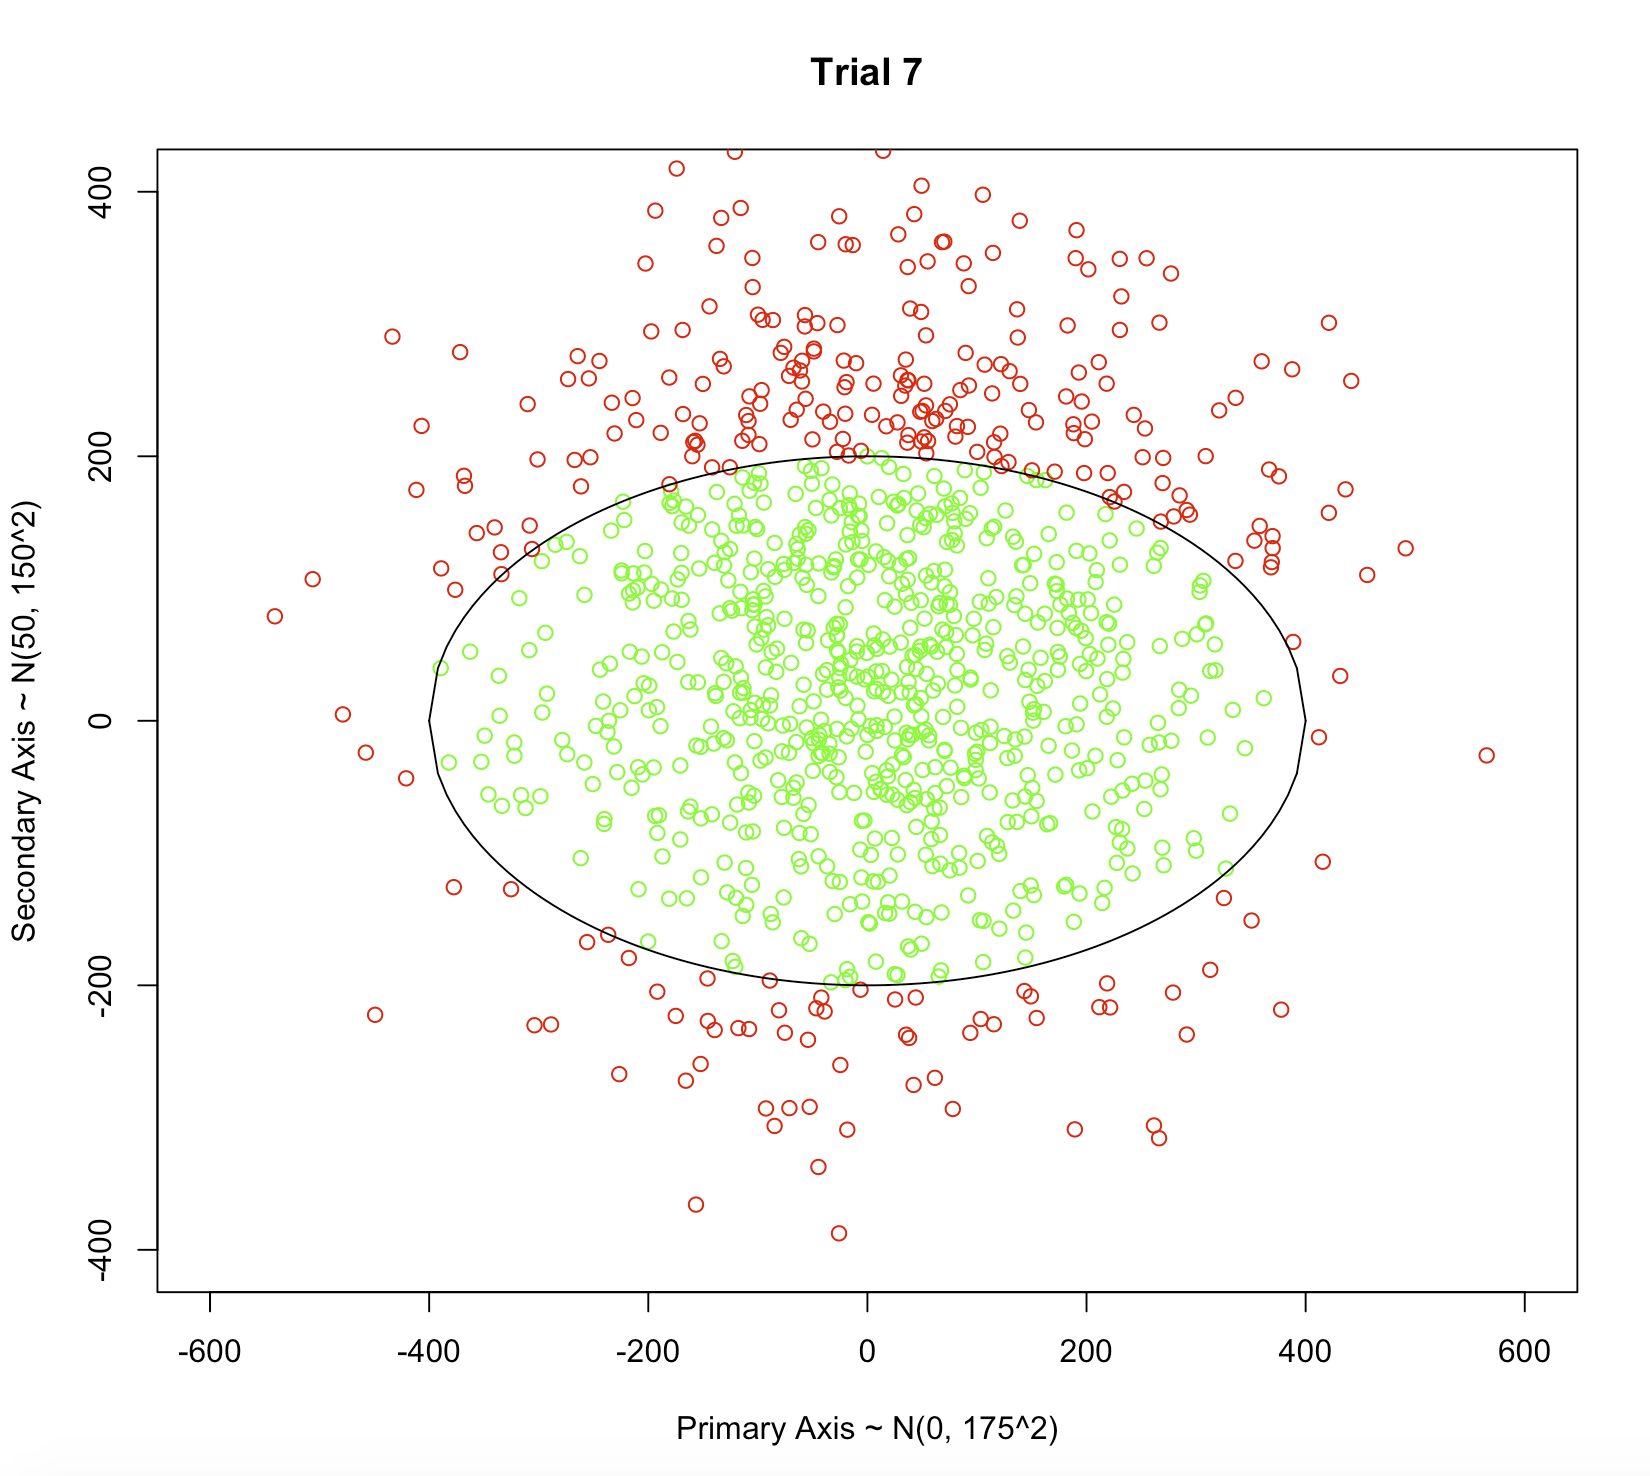
\includegraphics[scale=.35]{trial7}

\textbf{TRIAL 8}
\newline
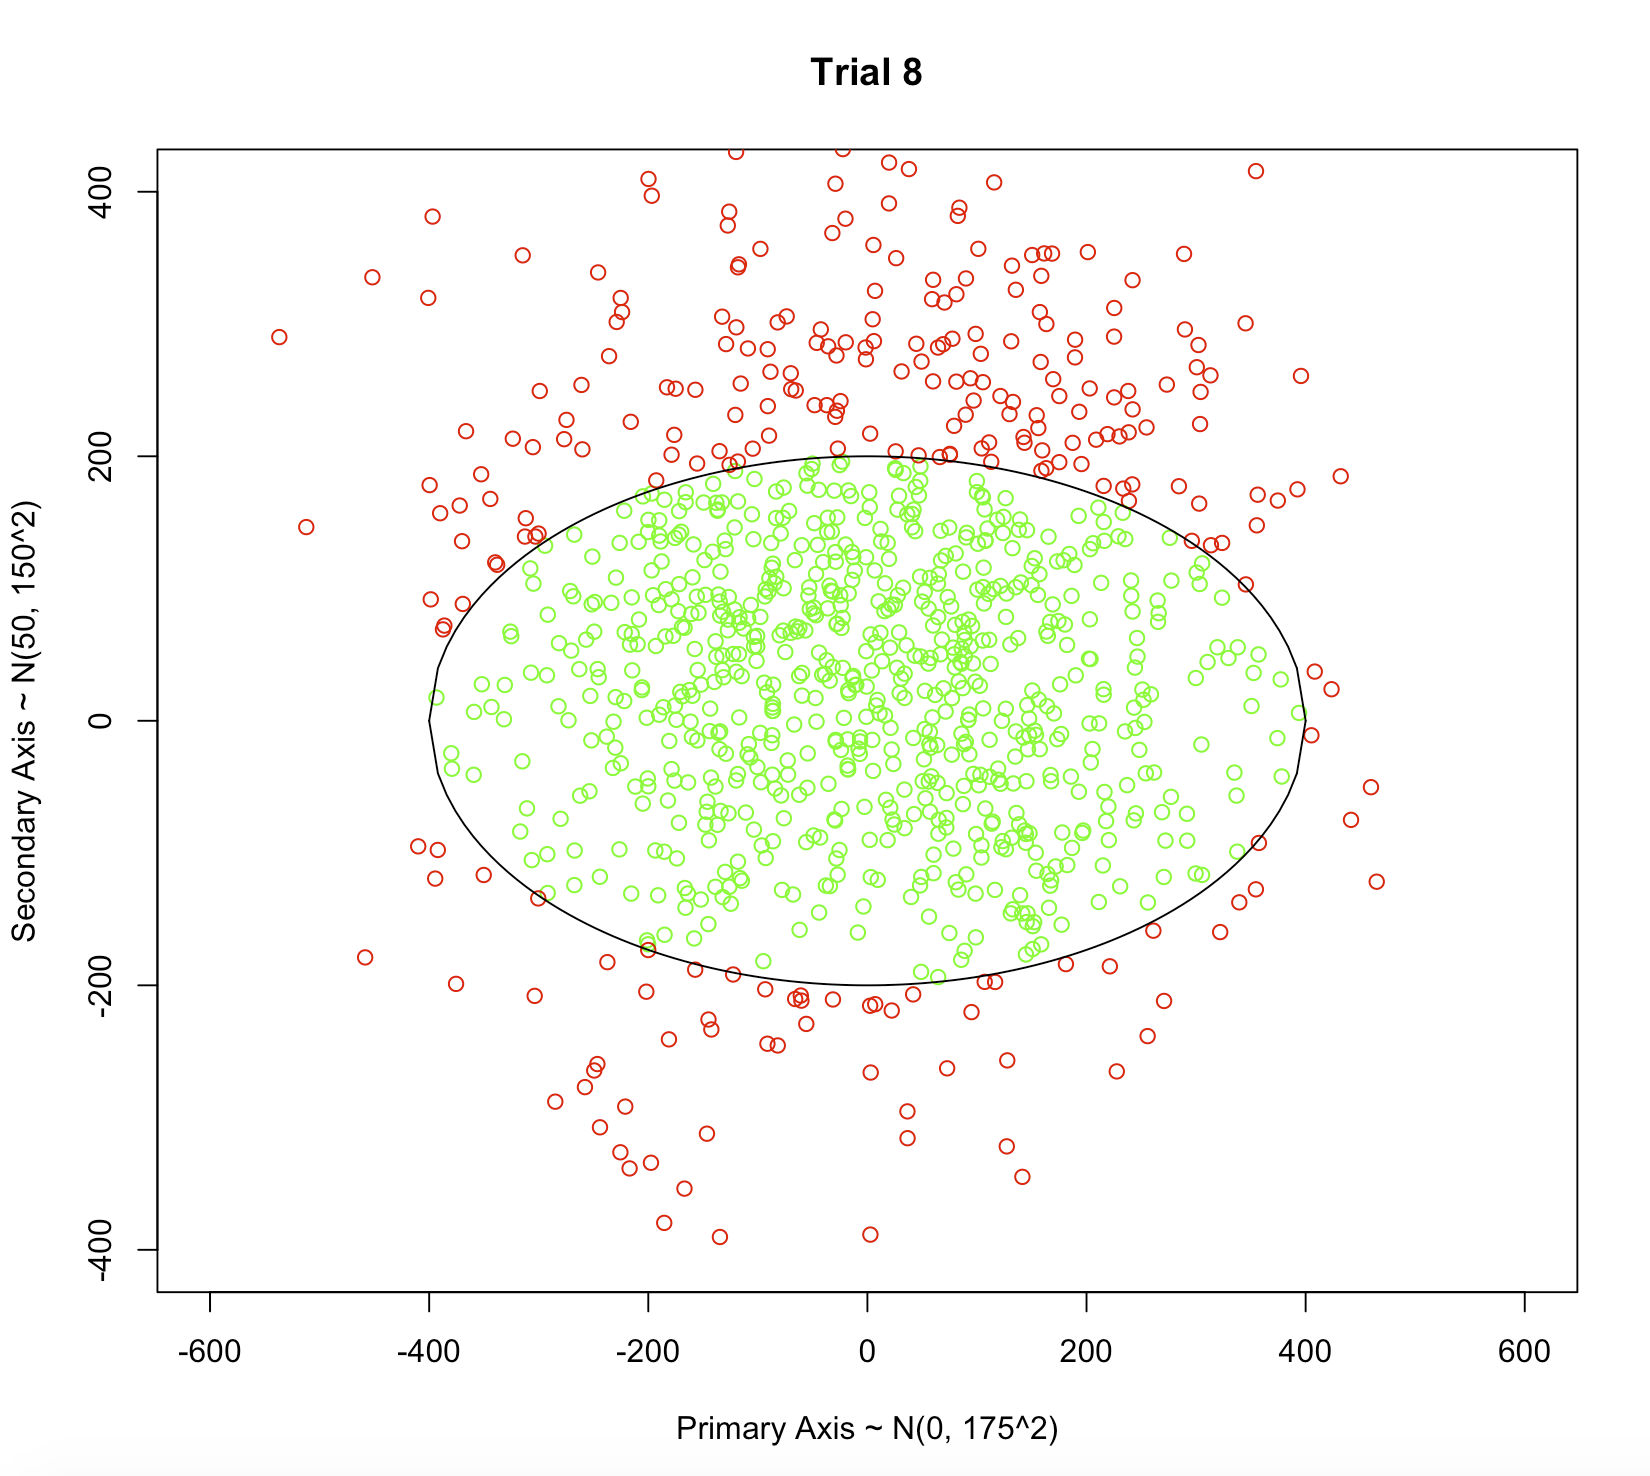
\includegraphics[scale=.35]{trial8}

\textbf{TRIAL 9}
\newline
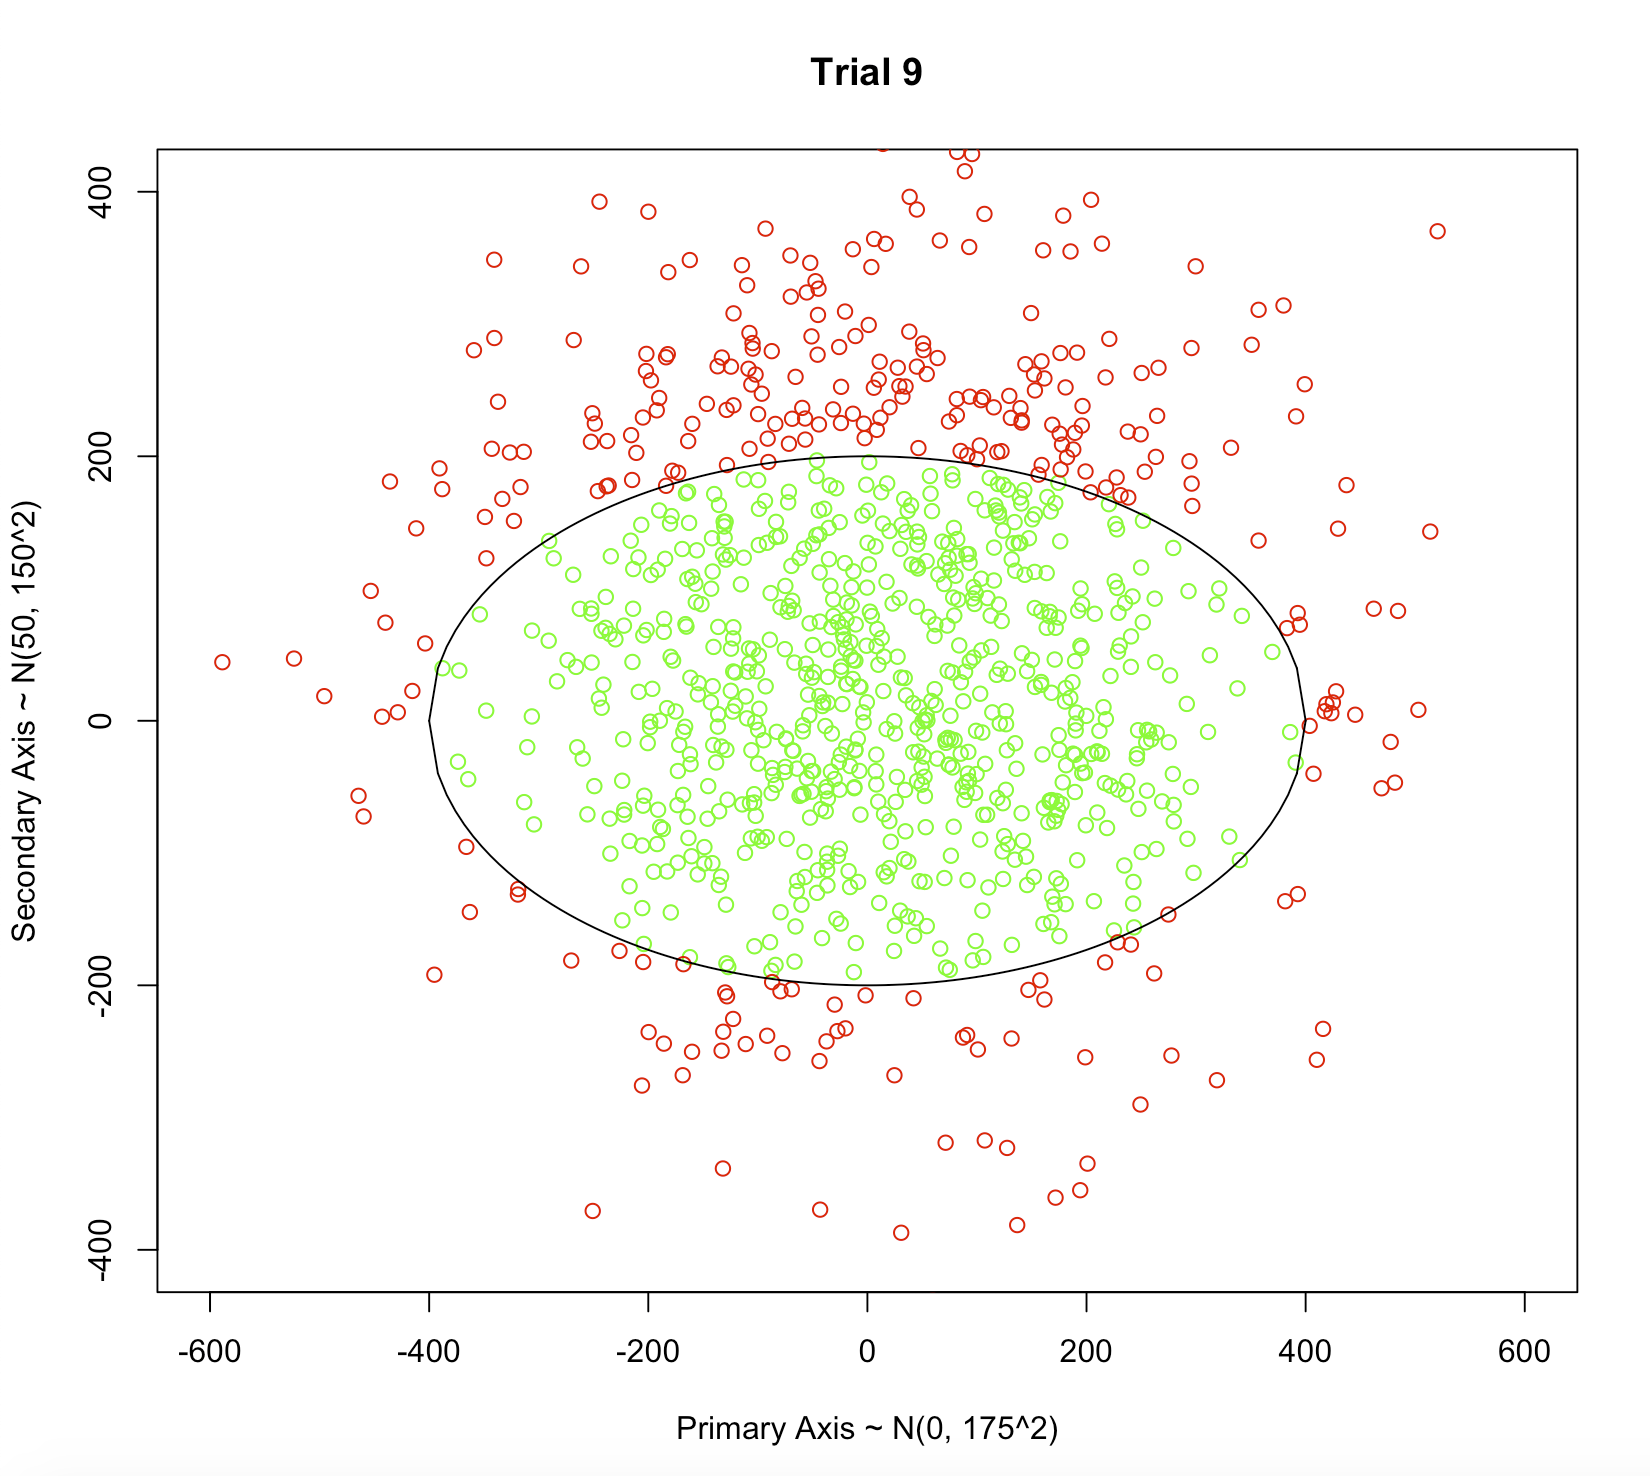
\includegraphics[scale=.35]{trial9}

\textbf{TRIAL 10}
\newline
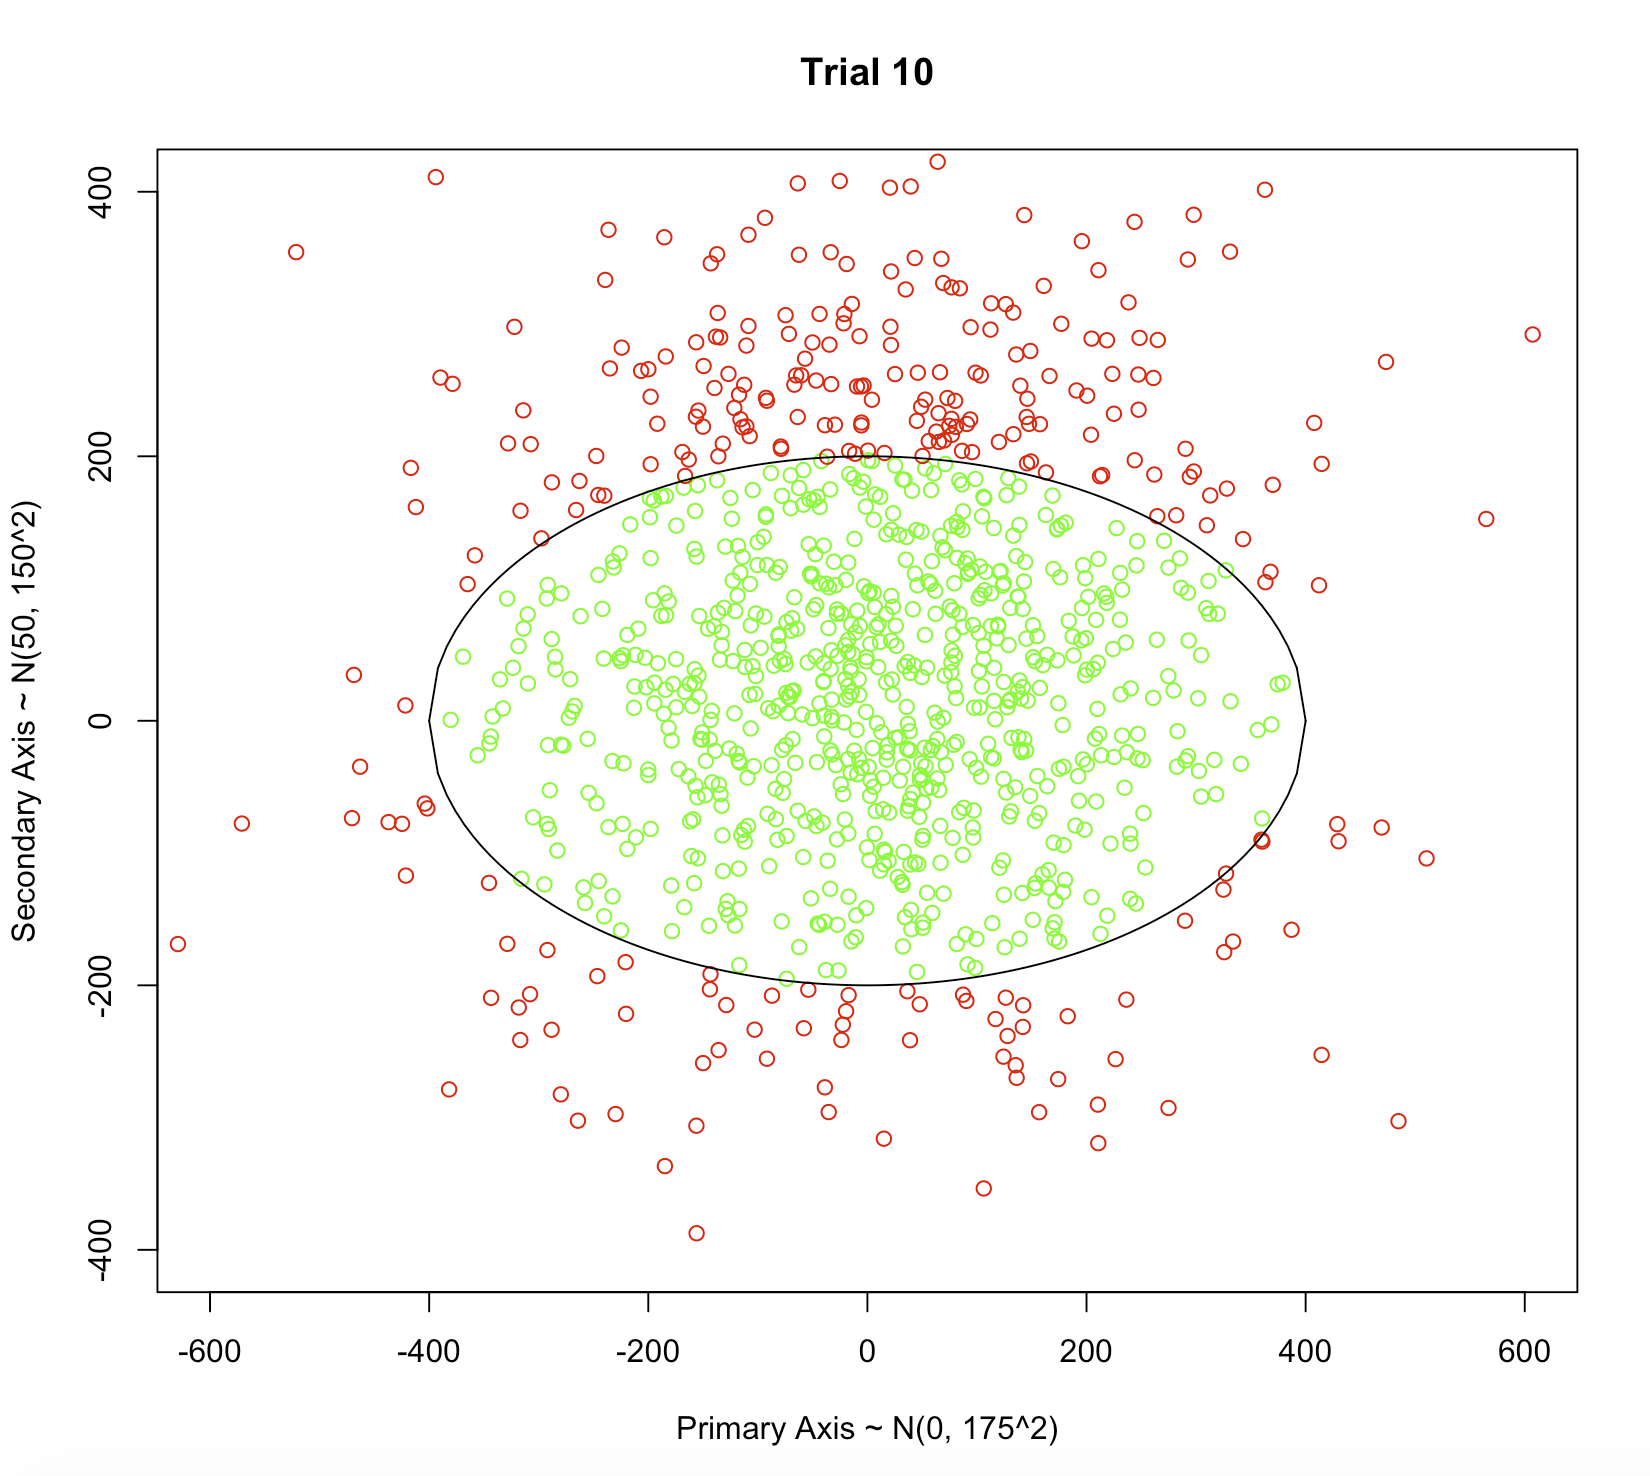
\includegraphics[scale=.35]{trial10}

\end{document}